\documentclass[12pt, openany]{report}
\usepackage[utf8]{inputenc}
\usepackage[T1]{fontenc}
\usepackage{amsmath,amsfonts,amssymb}
\usepackage{bm}
\usepackage{amssymb}
\usepackage{multicol}
\usepackage[a4paper,left=2.5cm,right=2.5cm,top=2.5cm,bottom=2.5cm]{geometry}
\usepackage[english]{babel}
\usepackage{algpseudocode}
\usepackage{algorithm}
\usepackage{libertine}
\usepackage{graphicx}
\usepackage{wrapfig}
\usepackage{float}
\usepackage{nicematrix}
\usepackage{enumitem}
\usepackage{amsthm}
\usepackage{pythonhighlight}
\usepackage[]{titletoc}
\usepackage{empheq}
\usepackage{titlesec}
\usepackage{mathpazo}
\usepackage{xfrac}
\usepackage{textcomp}
\usepackage{mathtools}
\usepackage{caption}
\usepackage{tabularray}
\usepackage{subcaption}
\usepackage[bottom]{footmisc}
\usepackage{pdfpages}
\usepackage{tikz}
\usetikzlibrary{automata, positioning}
\usepackage{tabularx}
\usepackage[skins]{tcolorbox}

\theoremstyle{definition}
\newtheorem{thm}{Theorem}[chapter]
\newtheorem{definition}[thm]{Definition}
\newtheorem{exmp}[thm]{Example} 
\newtheorem{lem}[thm]{Lemma}
\newtheorem{proposition}[thm]{Proposition}
\newtheorem{corollary}[thm]{Corollary}

\titleformat{\chapter}[display]
  {\normalfont\bfseries}{}{0pt}{\Huge}
\usepackage{hyperref}
\newcommand{\hsp}{\hspace{20pt}}
\newcommand{\HRule}{\rule{\linewidth}{0.5mm}}
\newcommand{\R}{\mathbb{R}}
\newcommand{\C}{\mathbb{C}}

\begin{document}


\begin{titlepage}
    \begin{sffamily}
    \begin{center}
        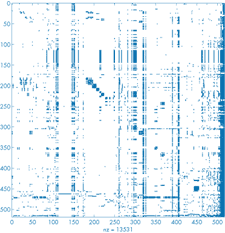
\includegraphics[scale=1]{img/page_de_garde.png} \\[1cm]
        \HRule \\[0.4cm]
        { \huge \bfseries LINMA2380 Matrix Computations \\[0.4cm] }
    
        \HRule \\[1.5cm]
        \textsc{\LARGE Simon Desmidt}\\[1cm]
        \vfill
        \vspace{2cm}
        {\large Academic year 2024-2025 - Q1}
        \vspace{0.4cm}
         
        
\includegraphics[width=0.15\textwidth]{img/epl.png}
        
        UCLouvain\\
    
    \end{center}
    \end{sffamily}
\end{titlepage}

\setcounter{tocdepth}{1}
\tableofcontents
\chapter{Reminders}
\section{Algebraic structures}
\begin{itemize}
    \item A semigroup is a set together with an associative binary operation \((E,+)\).
    \item A monoid is a semigroup with a neutral element.
    \item A group is a monoid in which every element has an inverse.
    \item A commutative group is a group whose binary operation is commutative.
    \item A ring is a triple \((E,+,\cdot)\) such that
    \begin{itemize}
        \item [\(\bullet\)] \((E,+)\) is a commutative group;
        \item [\(\bullet\)] \((E,\cdot)\) is a monoid;
        \item [\(\bullet\)] $\cdot$ is distributive with respect to \(+\).
    \end{itemize}
    \item An integral domain is a commutative ring in which the product of any two nonzero elements in nonzero : \[\forall x,y\in E, x,y\neq 0\qquad xy\neq 0\]. This implies that the equation \(ax=b\) with \(a\neq 0\) has at most one solution. 
    \item An Euclidean domain is an integral domain such that for every two elements in the domain, we can perform the Euclidean division: \[\forall (a_1,a_2), \quad \exists (q,r) : \quad a_1=a_2q+r \text{ with }r<a_2\]
    \item A field is a commutative ring \((E,+,\cdot)\) such that every \(a\in E\setminus \{0\}\) has a multiplicative inverse.
    \item \((K,E,+)\) is a module over the ring \((K,+,\cdot)\) if 
    \begin{itemize}
        \item [\(\bullet\)] \((E,+)\) is a commutative group;
        \item [\(\bullet\)] the external composition operation \(\cdot:K\times E\rightarrow E\) satisfies 
        \begin{itemize}
            \item \((a+b)\cdot x = a\cdot x+b \cdot x \qquad a\cdot (x+y) = a\cdot x+a\cdot y\)
            \item \(a\cdot (b\cdot x) = (a\cdot b)\cdot x\)
            \item \(1\cdot x = x\)
        \end{itemize}
    \end{itemize}
    \item If, in addition to that, \((K,+,\cdot)\) is a field, then \((K,E,+)\) is a vector space over \((K,+,\cdot)\).
    \item \((K,E,+,\cdot)\) is an algebra if 
    \begin{itemize}
        \item [\(\bullet\)] \((K,E,+)\) is a module or a vector space;
        \item [\(\bullet\)] the internal composition operation \(\cdot:E\times E\rightarrow E\) is bilinear.
    \end{itemize}
\end{itemize}
\section{Matrix algebras}
\subsection{Product}
Apart from the usual sum and product of two matrices, we can define the Hadamard and Kronecker products :
\begin{itemize}
    \item Hadamard : \[A_{m\times n}\odot B_{m\times n} \coloneqq [a_{ij}\cdot b_{ij}]_{i,j=1}^{m,n}\]
    \item Kronecker : \[A \otimes B \coloneqq \begin{bmatrix}
        a_{11}B & \dots & a_{1n}B\\
        \vdots & \ddots & \vdots \\
        a_{m1}B & \dots & a_{mn}B\\
    \end{bmatrix}\]
\end{itemize}
A square matrix \(A\in \mathbb{C}^{n\times n}\) is said normal if \(AA^* = A^*A\). In the real case, it is said to be orthogonal and \(*\) is equivalent to the transpose. Furthermore, it is said to be unitary if it satisfies the relations \(AA^* = I_n = A^*A\). 
\subsection{Determinant}
We define the quasi-diagonals of a matrix as the \(n\)-tuples of elements of a matrix \(A\), \(a_{1j_1,2j_2,\dots,nj_n}\) where the indices \(\textbf{j} = (j_1,\dots,j_n)\) constitute a permutation of the set \(\{1,2,\dots,n\}\). Thus a quasi-diagonal consists of \(n\) elements of the matrix \(A\) in such a way that no two of them lie in the same row or column of \(A\). For each quasi-diagonal, we define the parity \(t(\textbf{j})\). It is the number of inversions \(j_k>j_p\) for \(k<p\) in \(\textbf{j}\).
\begin{itemize}
    \item With the notation above, we define the determinant of a square matrix \(A_{n\times n}\) as \[\det (A) = \sum_\textbf{j} (-1)^{t(\textbf{j})} a_{1j_1}\cdot a_{2j_2}\cdot \dots \cdot a_{nj_n}\]
\end{itemize}
The determinant has the following properties :
\begin{itemize}
    \item The determinant is multilinear in the rows of \(A\) : \[\det \begin{bmatrix}
        a_{1:}\\ \vdots \\ b_{k:} +\lambda c_{k:} \\ \vdots \\ a_{n:}
    \end{bmatrix} = \det \begin{bmatrix}
        a_{1:}\\ \vdots \\ b_{k:} \\ \vdots \\ a_{n:}
    \end{bmatrix} + \det \begin{bmatrix}
        a_{1:}\\ \vdots \\ \lambda c_{k:} \\ \vdots \\ a_{n:}
    \end{bmatrix}\]
    \item The determinant is alternating in the rows of \(A\) : for \(i\neq j\), \(a_{i:}=a_{j:} \Longrightarrow \det(A) = 0\)
    \item \(\det(I_n) = 1\), where \(I_n\) is the identity matrix.
\end{itemize}
\begin{minipage}{.5\textwidth}
\begin{itemize}
    \item \(\det\begin{bmatrix}
        a_{1:} \\ \vdots \\ a_{i:} \\ \vdots \\ a_{j:} \\ \vdots \\ a_{n:}
    \end{bmatrix} = - \det\begin{bmatrix}
        a_{1:} \\ \vdots \\ a_{j:} \\ \vdots \\ a_{i:} \\ \vdots \\ a_{n:}
    \end{bmatrix}\)
\end{itemize}
\end{minipage}
\begin{minipage}{.5\textwidth}
\begin{itemize}
    \item \(\det\begin{bmatrix}
        a_{1:} \\ \vdots \\ a_{i:} +\lambda a_{j:}\\ \vdots \\ a_{n:}
    \end{bmatrix} = \det\begin{bmatrix}
        a_{1:} \\ \vdots \\ a_{i:} \\ \vdots \\ a_{n:}
    \end{bmatrix}\)
\end{itemize}
\end{minipage}
\begin{itemize}
    \item \(\det (\lambda A)=\lambda^n \det(A)\)
    \item for \(i\neq j\), \(a_{i:} = \lambda a_{j:} \Longrightarrow \det(A) = 0\)
    \item \(\det(A^T) = \det(A)\)
    \item \(\det(A^*) = \overline{\det(A)}\), if \(A\in \mathbb{C}^{n\times n}\)
    \item [\(\rightarrow\)] N.B.: any property of the determinant established for the rows of matrices also holds for the columns.
    \item The minor \(A_{(kl)}\) of dimension \(n-1\) of a matrix \(A_{n\times 
 n}\) is the determinant of the submatrix obtained by removing the \(k\)the row and the \(l\)th column. From this, we can note the determinant as a linear combination of the elements of a row or column : \[\det(A) = a_{1j}A_{1j}^c + a_{2j}A_{2j}^c + \dots + a_{nj}A_{nj}^c \\ \det(A) = a_{i1}A_{i1}^c + a_{i2}A_{i2}^c + \dots + a_{in}A_{in}^c\] where the coefficient \(A_{kl}^c\) is called the cofactors of the corresponding element \(a_{kl}\)\footnote{\(A_{kl}^c = (-1)^{k+l}A_{(kl)}\).}
\end{itemize}
\subsubsection{Laplace and Binet-Cauchy relations}
For the pairs of \(p\)-tuples \[\textbf{i}_p \coloneqq (i_1,\dots,i_p)\text{ and }\textbf{j}_p\coloneqq (j_1,\dots j_p)\] satisfying \[1\le i_1<\dots<i_p\le n\text{ and } 1\le j_1<\dots<j_p\le n\] we define the minors of order \(p\) of \(A\) as 
\begin{equation}
    A\begin{pmatrix}
        \textbf{i}_p\\ \textbf{j}_p
    \end{pmatrix} \coloneqq \det[a_{i_k,j_l}]_{k,l=1}^p
\end{equation}
We also define the complementary cofactors of \(A\) as 
\begin{equation}
    A^c\begin{pmatrix}
        \textbf{i}_p\\ \textbf{j}_p
    \end{pmatrix} \coloneqq (-1)^s A\begin{pmatrix}
        \textbf{i}_p^c\\ \textbf{j}_p^c
    \end{pmatrix}
\end{equation}
where \(s = \sum_{k=1}^p(i_k+j_k)\) and \(\textbf{i}_p^c\) is the set complement of \(\textbf{i}_p\) (same for \(\textbf{j}_p\)). \\
\underline{Laplace Theorem:}\\
Let \(A\) be a matrix of dimensions \(n\times n\) and \(\textbf{i}_p\) be a \(p\)-tuple of rows (and \(\textbf{j}_p\) for the columns). Then, \(\det(A)\) is equal to the sum of the products of all possible minors located in these rows/columns with their complementary cofactors:
\begin{equation}
    \begin{cases}
        \det(A) = \sum_{\textbf{j}_p}A\begin{pmatrix}
            \textbf{i}_p\\\textbf{j}_p
        \end{pmatrix} A^c\begin{pmatrix}
            \textbf{i}_p\\\textbf{j}_p
        \end{pmatrix}\\
        \det(A) = \sum_{\textbf{i}_p}A\begin{pmatrix}
            \textbf{i}_p\\\textbf{j}_p
        \end{pmatrix} A^c\begin{pmatrix}
            \textbf{i}_p\\\textbf{j}_p
        \end{pmatrix}\\
    \end{cases}
\end{equation}
\underline{Binet-Cauchy Theorem:}\\
Let \(\textbf{m}\) be the \(m\)-tuple \((1,\dots,m)\). Let \(A\) and \(B\) be matrices of dimensions \(m\times n\) and \(n\times m\) respectively. If \(m\le n\), then 
\begin{equation}
    \det(AB) = \sum_{\textbf{j}_m} \det A\begin{pmatrix}
        \textbf{m}\\ \textbf{j}_m
    \end{pmatrix} \det B\begin{pmatrix}
        \textbf{j}_m\\ \textbf{m}
    \end{pmatrix}
\end{equation}
\subsection{Inverse and rank}
\begin{itemize}
    \item The adjugate matrix of a square matrix \(A_{n\times n}\) is defined as \[adj(A) \coloneqq [A_{ji}^c]_{i,j=1}^n\]
\end{itemize}
Then, for every square matrix \(A_{n\times n}\), we have
\begin{equation}
    A\cdot adj(A) = \det(A) I_n = adj(A)\cdot A
\end{equation}
Every matrix \(A_{m\times n}\) whose elements belong to a field \(\mathcal{F}\) can be brought to the following form by means of invertible (or elementary) transformations of rows and columns:
\begin{equation}
    RAQ = \begin{pNiceArray}{cc|c}
    I_r && 0_{r\times (n-r)}\\
  \hline
  0_{(m-r)\times r} && 0_{(m-r)\times (n-r)}\\
\end{pNiceArray}
\end{equation}
The rank of a matrix \(A_{m\times n}\) whose elements belong to a field \(\mathcal{F}\) is equal to the largest size of its nonzero minors. As a corollary, any non-singular matrix whose elements belong to a field \(\mathcal{F}\) can be written as a product of elementary transformations.\\

\underline{Schur complement:}\\
Let \(A_{n\times n}\) be an invertible submatrix of the matrix \[M_{(n+p)\times (n+m)} = \begin{pmatrix}
    A & B\\ C & D\\
\end{pmatrix}\]
Then the rank of \(M\) satisfies 
\begin{equation}
    rank(M) = n + rank(D-CA^{-1}B)
\end{equation}
And the matrix \(D-CA^{-1}B\) is called the Schur complement of \(M\). 
\chapter{QR form}
TODO
\chapter{Unitary transformations and SVD}
\section{Introduction and definitions}
\begin{itemize}
    \item A unitary matrix is a matrix \(U\in \C^{n\times n}\) such that \(U^*U=I\), i.e. its column are orthogonal.
    \item An isometry is a matrix \(U\in \C^{m\times n}\), \(m\neq n\), such that \(U^*U=I\). We have \(\lVert Ux\rVert =\lVert x \rVert\). 
\end{itemize}
\section{Diagonalization by unitary transformations}
The goal here is to have a matrix decomposition of the form 
\begin{equation}
    A = R\begin{pmatrix}
        I_r & 0\\ 0& 0 \\
    \end{pmatrix}Q^{-1}
\end{equation}
for any arbitrary matrix \(A_{m\times n}\), and with \(R,Q\) being unitary (if \(A\) is complex) or orthogonal (if \(A\) is real). We limit ourselves here to transformation matrices that are isometries\footnote{To define.}. This means that the invariants that we obtain characterize the way the matrix act on the norm of vectors. 
\begin{thm}
    Every Hermitian\footnote{\(A=A^*\)} matrix \(A\in \C^{n\times n}\) can be diagonalized by a unitary transformation \(U\in \C^{n\times n}\):
    \begin{equation}
        U^*AU = \begin{pmatrix}
            \lambda_1 & 0 & \dots & 0\\
            0&\ddots &\ddots \vdots \\
            \dots & \ddots & \ddots & 0\\
            0 & \dots & 0 & \lambda_n\\
        \end{pmatrix}
    \end{equation}
    with \(\lambda_i\in \R\).
\end{thm}
\begin{thm} 
    The eigenvalues of a Hermitian matrix \(A\in \C^{n\times n}\) are invariant under unitary similarity transformations:
    \begin{equation}
        B=U^*AU
    \end{equation}
    Every class of equivalence defined by this transformation group has a unique canonical representative which is the diagonal matrix \(\Lambda\) with the eigenvalues of \(A\) decreasing along the diagonal.
\end{thm}
\begin{thm}[\textbf{Singular Value Decomposition}]
    For every matrix \(A\in \C^{m\times n}\), there exist unitary transformations \(U\in \C^{m\times m}\) and \(V\in \C^{n\times n}\) such that 
    \begin{equation}
        A=U\Sigma V^* \qquad \Sigma = \begin{pNiceArray}{ccc|c}
            \sigma_1 &        & 0                  &  \\
                     & \ddots &                    & 0_{r\times (n-r)}\\
            0        &        & \sigma_r           &  \\ \hline
                     & 0_{(m-r)\times r} & & 0_{(m-r)\times (n-r)}\\
          \end{pNiceArray}
        \end{equation}
    with real positive singular values \(\sigma_1\ge \dots \ge \sigma_r > 0\). The value \(r\) and the \(r\)-tuple \((\sigma_1,\dots,\sigma_r)\) are uniquely defined and, as a consequence, the matrix \(\Sigma\) constitutes a canonical form under unitary transformations, i.e. under transformations of the form \(B = \tilde U^* A\tilde V\). Where \(\tilde U, \tilde V\) are two unitary matrices. 
\end{thm}
\underline{Properties:}
\begin{itemize}
    \item If the matrix \(A\) is real, \(U,V\) are orthogonal matrices;
    \item The transformations \(U,V\) diagonalize the matrices \(AA^*\) and \(A^*A\) respectively, since \(U^*AA^*U = \Sigma \Sigma^T\), \(V^*A^*AV=\Sigma^T\Sigma\), and the columns of \(U,V\) are the eigenvectors of \(AA^*\) and \(A^*A\) respectively.
    \item The transformations \(U,V\) are not uniquely defined. 
\end{itemize}
\section{Linear operator point of view}
We define the compact SVD form: \(A=U_1\Sigma_rV_1^*\), to have \(\Sigma_r\) invertible. In this form, \(\Sigma_r\) is \(r\times r\), \(r\) being the number of nonzero singular values. \(U_1\) contains the \(r\) first columns of \(U\) and \(V_1^*\) the \(r\) first lines of \(V^*\). The other columns (resp. rows) of \(U\) (resp. \(V\)) are denoted by the matrix \(U_2\) (resp. \(V_2^*\)). 
\begin{definition}
    If \(\mathcal{X}_1,\mathcal{X}_2\) are subspaces of \(\R^n\) such that their intersection is the origin, then we note \(\mathcal{X}_1\oplus \mathcal{X}_2\)=\(\mathcal{X}_1+\mathcal{X}_2\) the direct sum of the two spaces. 
\end{definition}
Any vector \(x\in \mathcal{X}_1\oplus \mathcal{X}_2\) has a unique decomposition \(x=x_1+x_2, \:x_i\in \mathcal{X}_i\). \\
For the SVD, we have 
\begin{align}
    \mathcal{X}_1 = Im(V_1) & \qquad \qquad \mathcal{X}_2 = Im(V_2) = Ker(A)\\
    \mathcal{Y}_1 = Im(U_1) = Im(A) &\qquad  \qquad \mathcal{Y}_2 = Im(U_2)
\end{align}
\section{Polar decomposition - formal point of view}
Any matrix \(A_{n\times n}\) can be expressed in the following form:
\begin{equation}
    A = \underbrace{U\Sigma U^*}_{\eqcolon H_1}UV^* = H_1Q = H_1\exp(iH_2)
\end{equation}
with \(H_1\) a positive definite Hermitian matrix, \(Q\) unitary and \(H_2\) also Hermitian.
\section{Projectors and generalized inverses - algebraic point of view}
\begin{definition}
    A projector is a matrix \(P\in \C^{n\times n}\) such that \(P^2=P\). \\
    It is said to be orthogonal if \(\forall x,\: (Px)^*(x-Px) = 0\). 
\end{definition}
\begin{thm}
    Any projector \(P\) can be written \(P=XY^*\) with \(Y^*X=I_r\), \(r\) being the rank of \(P\). If \(P\) is orthogonal, then \(X=Y\). 
\end{thm}
\begin{itemize}
    \item \(Im(P) = Ker(P^\perp)\)
    \item \(P=P^*\)
\end{itemize}
\section{Least squares}
\begin{thm}
    Given a linear system \(Ax=y\), the generalized inverse \(A^I = V_1\Sigma_r^{-1}U_1^*\) gives \(x^* = A^I y\) the solution minimizing the norm of \(Ax-y\). If there are more than one such solution, it returns the one of smallest norm.
\end{thm}
\section{Unitarily invariant matrix norms - geometric point of view}
A matrix norm is unitarily invariant if, for every \(A\in \C^{m\times n}\), we have \(\lVert A\rVert = \lVert U^*AV\rVert\) if \(U,V\) are unitary.\\
The 2-norm and the Frobenius norm of \(A\in \C^{m\times n}\) are unitarily invariant.
\begin{equation}
    \lVert A \rVert _2 \coloneqq \sup_{x\neq 0}\frac{\lVert Ax \rVert _2}{\lVert x \rVert _2} \qquad \lVert A \rVert _F \coloneqq \left(\sum_{i,j} \lvert a_{i,j} \rvert^2 \right)^{1/2}
\end{equation}
\section{Canonical angles}
\begin{thm}
    Given two subspaces \(\mathcal{S}_i\subseteq \C^n\) (\(i=1,2\)), there exist orthonormal bases given by the columns of \(\Hat S_i\) respectively, and satisfying 
    \begin{equation}
        \Hat S_1^*\Hat S_2 = \begin{pNiceArray}{ccc|c}
            \sigma_1 & & 0 & \\
            & \ddots & & 0_{r\times (r_2-r)}\\
            0 & & \sigma_r & \\
            \hline
            & 0_{(r_1-r)\times r} & & 0_{(r_1-r)\times r_2-r}\\
        \end{pNiceArray} \qquad 1\ge \sigma_1 \ge \dots \ge \sigma_r>0
    \end{equation}
\end{thm}
\color{red} Add the paper sheet of notes.\color{black}
\section{Variational problems}
\begin{thm}
    For a Hermitian matrix $H\in \C^{n\times n}$, the Rayleigh quotient is defined as 
    \begin{equation}
        R(x) \coloneqq \frac{\langle Hx,x\rangle}{\langle x,x\rangle} = \frac{x^*Hx}{x^*x} \qquad x\neq 0\in \C^n
    \end{equation}
    The Rayleigh quotient of a Hermitian matrix $H\in \C^{n\times n}$ is real and satisfies 
    \begin{equation}
        \lambda_{\min}(H) \le R(x)\le \lambda_{\max}(H)
    \end{equation}
\end{thm}
Furthermore, supposing that $\lambda_1\ge \dots\ge \lambda_n$, we have
\begin{equation}
    \lambda_n=\min_{x\neq 0}R(x) \qquad \lambda_1 = \max_{x\neq 0}R(x)
\end{equation}
\begin{lem}
    Let $\mathcal{S}_j \subseteq \C^n$ be a subspace of dimension $j$. Then, it holds that 
    \begin{equation}
        \min_{x\neq 0\in \mathcal{S}_j} R(x)\le \lambda_j\qquad \max_{x\neq 0\in S_j}R(x)\ge \lambda_{n-j+1}
    \end{equation}
\end{lem}
\begin{thm}[Courant-Fisher]
    For any Hermitian matrix $H\in \C^{n\times n}$, the Rayleigh quotient $R(x)$ satisfies 
    \begin{equation}
        \lambda_j=\max_{\mathcal{S}_j} \min_{x\neq 0 \in \mathcal{S}_j} R(x)\qquad \lambda_{n-j+1}=\min_{\mathcal{S}_j} \max_{x\neq 0 \in \mathcal{S}_j} R(x)
    \end{equation}
\end{thm}
\begin{thm}
    The singular values of an arbitrary matrix $A\in \C^{m\times n}$ are given by 
    \begin{align}
        \sigma_j(A) & = \max_{\mathcal{S}_j}\min_{x\neq 0\in \mathcal{S}_j} \frac{\lVert Ax\rVert_2}{\lVert x\rVert_2}\\
        \sigma_{n-j+1}(A) & = \min_{\mathcal{S}_j}\max_{x\neq 0\in \mathcal{S}_j} \frac{\lVert Ax\rVert_2}{\lVert x\rVert_2}
    \end{align}
\end{thm}
The following theorem is a major application of the SVD, as it allows to store a matrix with much less information that it contains.
\begin{thm}
    Let $A\in \C^{m\times n}$ be a matrix of rank $r$. The best approximation of $A$ by a matrix $B\in \C^{m\times n}$ of rank $s<r$ satisfies
    \begin{equation}
        \min_{\text{rank}(B)\le s}\lVert A-B\rVert_2 =\sigma_{s+1}(A)
    \end{equation}
\end{thm}
\begin{thm}[Eckart-Young]
    Furthermore, the matrix $A$ from the last theorem also satisfies
    \begin{equation}
        \min_{\text{rank}(B)\le s}\lVert A-B\rVert _F^2 = \sigma_{s+1}^2 + \dots + \sigma_r^2
    \end{equation}
\end{thm}
\chapter{Eigenvalues, eigenvectors and similarity transformations}
The eigenvalues of a matrix are invariant under similarity transformations. The similiary transformations $A\rightarrow TAT^{-1}$ define an equivalence class of matrices and every matrix $A_T$ belonging to the similarity class of $A$ has the same eigenvalues. 
\begin{thm}[Schur]
    Every matrix $A\in \C^{n\times n}$ can be upper triangularized under unitary similarity transformations:
    \begin{equation}
        U^*AU = \begin{bmatrix}
            \lambda_1 & \times & \cdots & \times\\
            0 & \lambda_2 & \ddots & \vdots\\
            \vdots & \ddots & \ddots & \times\\
            0 & \dots & 0 & \lambda_n
        \end{bmatrix} \eqcolon A_S
    \end{equation}
    where the diagonal of $A_S$ consists of the eigenvalues of $A$.
\end{thm}
\begin{itemize}
    \item If $A$ is Hermitian, then $A_S$ is Hermitian, and thus diagonal and real. This is its canonical form.
    \item The eigenvalues in the Schur form can be ordered. 
    \item If $A\in \R^{n\times n}$, the eigenvalues and eigenvectors can be complex. Then, their complex conjugates are also eigenvalues and eigenvectors of $A$.
\end{itemize}
\begin{definition}
    A normal matrix is a square matrix $A\in \C^{n\times n}$ satisfying $AA^*=A^*A$.
\end{definition}
\begin{thm}
    A matrix $A\in \C^{n\times n}$ is normal if and only if it is diagonalizable under unitary similarity transformations: $A=U\Lambda U^*$.
\end{thm}
\section{Invariant subspaces}
\begin{definition}
    A subset $\mathcal{X}\subseteq \C^n$ is an invariant subspace under the operator $A\in \C^{n\times n}$ if $A\mathcal{X}\subseteq \mathcal{X}$.
\end{definition}
\begin{thm}
    Let $\mathcal{X}\subseteq \C^n$ be a subspace of dimension $k$. Let $X\in \C^{n\times k}$ be such that the columns of $X$ form a basis of $\mathcal{X}$, and let $X_c$ be a completion of $X$ such that $T\coloneqq [X|X_c]$ is non-singular. Then, the following three propositions are equivalent:
    \begin{itemize}
        \item $A\mathcal{X}\subseteq \mathcal{X}$;
        \item $AX=XA_{11}$;
        \item $T^{-1}AT=\begin{bNiceArray}{c|c}
            A_{11}& A_{12}\\
            \hline
            0_{(n-k)\times k} & A_{22}\\
        \end{bNiceArray}$
    \end{itemize}
    where $A_{11}\in \C^{k\times k}$, $A_{12}\in \C^{k\times (n-k)}$ and $A_{22}\in \C^{(n-k)\times (n-k)}$.
\end{thm}
\begin{thm}[Real Schur form]
    Every matrix $A\in \R^{n\times n}$ can be almost triangularized under real similarity transformations $U\in \R^{n\times n}$, and with blocks of dimension $1\times 1$ or $2\times 2$:
    \begin{equation}
        U^TAU = \begin{bmatrix}
            A_{11} & \times & \dots & \times\\
            & A_{22} & \ddots & \vdots\\
            &&\ddots & \times\\
            &&& A_{kk}\\ 
            \end{bmatrix} \qquad A_{ii}\in \R^{1\times 1}\cup \R^{2\times 2}
    \end{equation} 
\end{thm}
\section{Jordan canonical form}
\begin{thm}
    Every matrix $A\in \C^{n\times n}$ admits a block-diagonal form under similarity transformations:
    \begin{equation}
        T^{-1}AT = A_S = diag\{A_{11},\dots,A_{kk}\}
    \end{equation}
    where each block $A_{ii}$ has only one eigenvalue (with multiplicity possibly larger than 1).
\end{thm}
\begin{thm}
    Every matrix $A\in \C^{n\times n}$ can be transformed by similarity transformations into a block-diagonal form:
    \begin{equation}
        T^{-1}AT = diag\{J_1(\lambda),\dots,J_k(\lambda)\}
    \end{equation}
    where each $J_i(\lambda)\in \C^{n_i\times n_i}$ is a Jordan block:
    \begin{equation}
        J_i(\lambda) = \begin{bmatrix}
            \lambda & 1 &&&\\
            & \lambda & 1&&\\
            &&\ddots&\ddots&\\
            &&&\lambda & 1\\
            &&&&\lambda
        \end{bmatrix}
    \end{equation}
\end{thm}
\begin{corollary}
    Two matrices $A,B\in \C^{n\times n}$ are similar iff they have the same Jordan form.
\end{corollary}
For a real matrix $A\in \R^{n\times n}$, we can separate the real and imaginary parts of the eigenvalues: $\lambda = \alpha + \beta j$. Separating the eigenvectors $v=x+iy$:
\begin{equation}
    A \begin{bmatrix}
        x & y\\
    \end{bmatrix} = \begin{bmatrix} x & y\\\end{bmatrix} \begin{bmatrix}
    \alpha & \beta\\ -\beta & \alpha\\
    \end{bmatrix}
\end{equation}
\begin{corollary}
    Any real matrix $A\in \R^{n\times n}$ has an invariant space of dimensionn 1 or 2:
    \begin{equation}
        \begin{bmatrix}
            \alpha & \beta & 1 & 0 &&\\
            -\beta & \alpha & 0 & 1&&\\
            & & \alpha & \beta & 1& 0&& \\
            & & -\beta & \alpha & 0 & 1&&\\
            &&&&& \ddots & \ddots &\\
            &&&&&& 1&0\\
            &&&&&& 0&1\\
            &&&&&& \alpha & \beta\\
            &&&&&& -\beta & \alpha
        \end{bmatrix}
    \end{equation}
\end{corollary}
\begin{definition}
    Given a polynomial $p(x) = p_0+p_1x+ \dots + p_d x^d$, we define the matrix polynomial $p(A) = p_0 I+p_1A+ \dots + p_d A^d$.
\end{definition}
\begin{thm}
    If $A=TJT^{-1}$, $p(A)=Tp(J)T^{-1}$, and thus 
    \begin{equation}
        \lambda_i(p(A)) = p(\lambda_i(A))
    \end{equation}
\end{thm}
\begin{corollary}
    The characteristic polynomial of $A$ satisfies $\chi(A)=\prod_i (A-\lambda_iI)^{m_i}=0$, with $m_i$ the algebraic multiplicity of the eigenvalue $\lambda_i$.
\end{corollary}
\begin{thm}\textbf{(Bendixson)}
    The eigenvalues $\alpha+\beta j$ of a matrix $A\in \C^{n\times n}$  are in the rectangle 
    \begin{align}
        \lambda_{\min} \left(\frac{A+A^*}{2}\right) \le \alpha \le \lambda_{\max} \left(\frac{A+A^*}{2}\right)\\
        \lambda_{\min} \left(\frac{A-A^*}{2j}\right) \le \beta \le \lambda_{\max} \left(\frac{A-A^*}{2j}\right)
    \end{align}
\end{thm}
\begin{thm}
    Let $A\in \C^{n\times n}$. Its eigenvalues are all in the union of the Gershgorin circles: 
    \begin{equation}
        |z-a_{pp}| \le \sum_{k\neq p} |a_{pk}|
    \end{equation}
\end{thm}
\chapter{Polynomial matrices}
\section{Group of elementary matrices}
\begin{enumerate}
    \item Permutations: $P$ such that $P^T = P^{-1}$;
    \item Eliminations: $(I+p(x) E_{ij})^{-1} = I-p(x)E_{ij}$ where $E_{ij}$ is such that $e_{ij} = 1$ and all other elements are 0;
    \item Scaling matrices : The identity with a polynomial on one of the term of the diagonal. 
\end{enumerate}
Type I, II, and III with a constant polynomial are unimodular matrices. \\
\section{Smith form}
\begin{definition}
    A polynomial matrix $E(\lambda)\in \C^{n\times n}[\lambda]$ is unimodular if its determinant is a nonzero constant.
\end{definition}
From this it comes that the invertible polynomial matrices are exactly the unimodular matrices. 
\begin{algorithm}[H]
    \caption{Euclide's algorithm}
    \begin{algorithmic}[1]
        \State Input: $a\ge b\in \mathbb{Z}$.
        \State Output: GCD(a,b).
        \State $a = bq_1+r_1$ \\
        $i=1$;\\
        $r_0 = b$;\\
        Repeat if $r_i\neq 0$;\\
        If $r_i = 0$, $r_{i+1} \coloneqq r_{i-1}-r_i a_{i+1}$.
    \end{algorithmic}
\end{algorithm}
\begin{lem}
    The Euclide algorithm terminates in finite time $T$, with $r_T=0$ and $r_{T-1} = GCD(a,b)$. 
\end{lem}
\begin{thm}\textbf{Euclid-Stevin}
    For every two polynomials $a(\lambda),b(\lambda)\in \C[\lambda]$, there exists a unimodular transformation $U(\lambda)\in \C^{n\times n}[\lambda]$ such that 
    \begin{equation}
        \begin{bmatrix}
            a(\lambda)\\ b(\lambda)\\
        \end{bmatrix} = U(\lambda)\begin{bmatrix}
            d(\lambda)\\ 0\\
        \end{bmatrix}
    \end{equation}
    where $d(\lambda)$ is the greatest common divisor (gcd) of $a(\lambda)$ and $b(\lambda)$.
\end{thm}
\begin{corollary}
    For every $n$ polynomials $p_1(\lambda),\dots,p_n(\lambda)\in \C[\lambda]$, there exists a unimodular transformation $Q(\lambda)\in \C^{n\times n}[\lambda]$ such that
    \begin{equation}
        Q(\lambda) \begin{bmatrix}
            p_1(\lambda)\\ \vdots\\ p_n(\lambda)\\
        \end{bmatrix} = \begin{bmatrix}
            d(\lambda) \\ 0 \\ \vdots \\ 0 \\
        \end{bmatrix}
    \end{equation}
    where $d(\lambda)$ is the gcd of $p_1(\lambda),\dots,p_n(\lambda)$.
\end{corollary}
\begin{thm}\textbf{Hermite}
    Every polynomial matrix $P(\lambda)\in \C^{m\times n}[\lambda]$ can be transformed into a quasi-triangular form 
    \begin{equation}
        M(\lambda)P(\lambda)N = \begin{pNiceArray}{ccc|ccc}
            p_1(\lambda) & \dots & \times & \times & \dots & \times \\
             & \ddots & \vdots & \vdots & & \vdots \\
            & & p_r(\lambda) & \times & \dots & \times \\ \hline 
            &0_{(m-r)\times r} & && 0_{(m-r)\times (n-r)}&\\
        \end{pNiceArray}
    \end{equation}
    where $M(\lambda)\in \C^{m\times m}[\lambda]$ is unimodular and $N\in \R^{n\times n}$ is a permutation matrix.
\end{thm}
\begin{proposition}
    Let $P\in\mathbb{Z}^{n\times n}$, $M,N$ unimodular and $a\in \mathbb{Z}$. All $i\times i$ minors of $P$ are divisible by $a$ iff all minors of $MPN$ are divisible by $a$.
\end{proposition}
\begin{thm}\textbf{Smith}
    Every polynomial matrix $P(\lambda)\in \C^{m\times n}[\lambda]$ can be reduced by unimodular transformations $M(\lambda)\in \C^{m\times m}[\lambda]$ and $N(\lambda)\in \C^{n\times n}[\lambda]$ to a quasi-diagonal form
    \begin{equation}
        M(\lambda)P(\lambda)N(\lambda) = \begin{pNiceArray}{ccc|ccc}
            e_1(\lambda) & \dots & \times & & & \\
             & \ddots & \vdots & & 0_{r\times (n-r)} & \\
            & & e_r(\lambda) & & &\\ \hline 
            &0_{(m-r)\times r} & & & 0_{(m-r)\times (n-r)}&\\
        \end{pNiceArray}
    \end{equation}
    where $e_i(\lambda)$ divides $e_{i+1}(\lambda)$, which we denote $e_i(\lambda)|e_{i+1}(\lambda)$ ($i=1,\dots,r-1$). 
\end{thm}
\begin{thm}
    Let $i\le k\le n$. 
    \begin{equation}
        \prod_{1\le j\le k}e_j = GCD\text{ of all minors of size }k
    \end{equation}
    This means that the Smith form is canonical. 
\end{thm}
\begin{definition}
    The normal rank of a polynomial matrix $P(\lambda)\in \C^{m\times n}[\lambda]$ is the order of its largest nonzero minor. 
\end{definition}
\begin{itemize}
    \item [$\rightarrow$] Note: the Smith form is a canonical form under the group of unimodular transformations on the left and on the right. These transformations are equivalences, and two polynomial matrices are thus equivalent iff they have the same Smith form. 
\end{itemize}
\subsection{Smith form of a Jordan block}
\begin{lem}
    The Smith form of $\lambda I-A$ is the Smith form of $\lambda I-J_A$, $J_A$ being the Jordan form of $A$. 
\end{lem}
\begin{proposition}
    The Smith form of a Jordan block of size $n$ $\begin{pmatrix}
        \lambda-\lambda_i & 1 & & & \\
        & \lambda-\lambda_i & 1 & & \\
        &&\ddots&\ddots&\\
        &&&\lambda-\lambda_i & 1\\
        &&&&\lambda-\lambda_i
    \end{pmatrix}$ is \begin{equation}
        \begin{pmatrix}
            1& \\
            & 1 & \\
             & & \ddots & \\
            & & & (\lambda-\lambda_i)^n\\
        \end{pmatrix}
    \end{equation}
    For a Jordan matrix with several blocks of different sizes $n_j$ with the same eigenvalue, the Smith form is 
    \begin{equation}
        \begin{pmatrix}
            1 & \\
            & 1 &\\
            && \ddots & \\
            & & & (\lambda-\lambda_i)^{n_1}\\
            & & & & (\lambda-\lambda_i)^{n_2}\\
            & & & & & \ddots \\
            & & & & & & (\lambda-\lambda_i)^{n_k}\\
        \end{pmatrix}
    \end{equation}
\end{proposition}
\begin{thm}
    Let $A\in \C^{n\times n}$. The Smith form of $\lambda I-A$ is $diag(e_1(\lambda),e_2(\lambda),\dots, e_n(\lambda))$, where $e_{n-k+1}(\lambda)$ contains a factor $(\lambda-\lambda_i)^d$. if there are more than $k$ Jordan blocks of eigenvalue $\lambda_i$ and $d$ is the size of the $k$th largest Jordan block.
\end{thm}
\chapter{Nonnegative matrices}
\begin{definition}
    A nonnegative matrix $A$ is such that all its entries are nonnegative.
\end{definition}
\begin{definition}
    A nonnegative matrix $A\in \R_+^{n\times n}$ is irreducible if $(I+A)^{n-1} >0$.
\end{definition}
\begin{definition}
    A nonnegative matrix $A\in \R_+^{n\times n}$ is primitive if there exists $m\in \mathbb{Z}_+$ such that $A^m>0$.
\end{definition}
\begin{thm}
    In the case of $A$ irreducible, this theorem is referred as the Perron-Frobenius theorem.
    \begin{figure}[H]
        \centering
        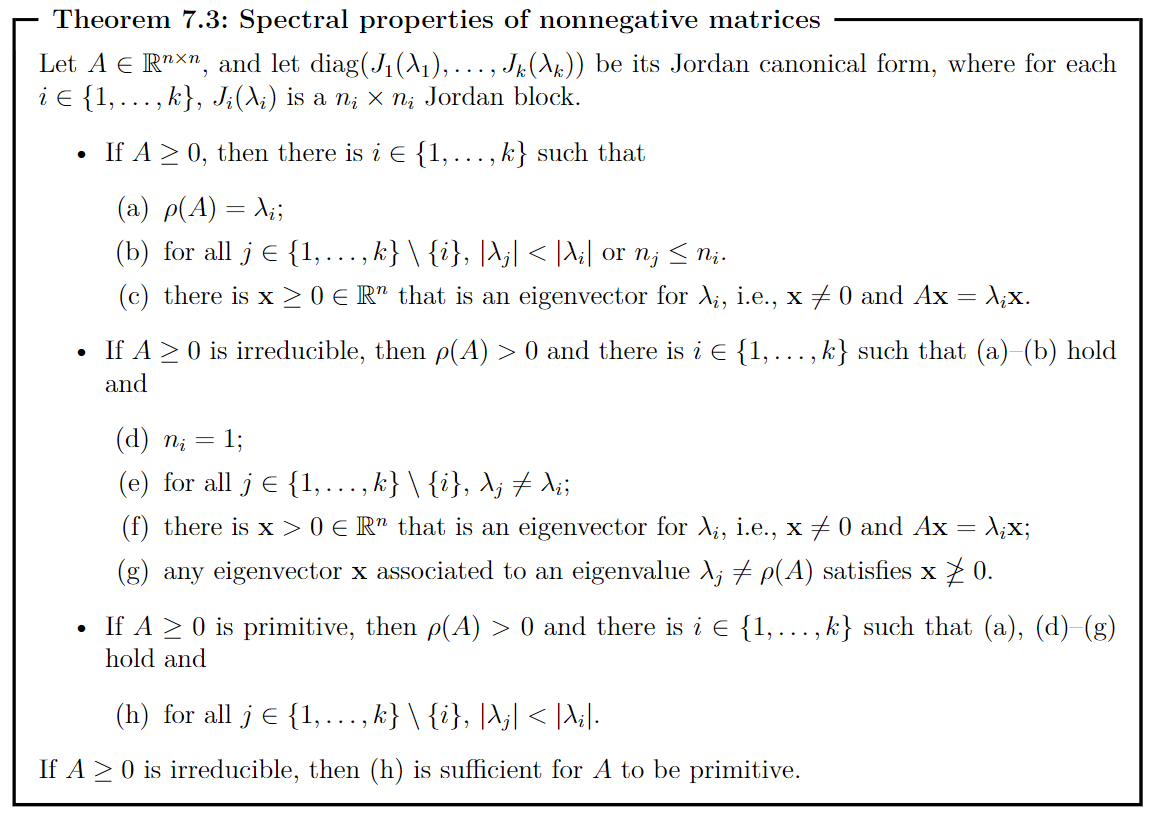
\includegraphics[width=\textwidth]{img/nonnegative_matrices.png}
    \end{figure}
\end{thm}
\begin{thm}
    $Ax$ is monotonous in $x$ if $x\ge x'\Longrightarrow Ax\ge Ax'$. If, for some $x$, $Ax\ge Mx$, then $A^tx\ge M^tx$ and $|\lambda_1(A)|\ge M$.
\end{thm}
\begin{proposition}
    If $A^k>0$ for some $k$, then the optimal $x^*$ in 
    \begin{equation}
        \max_{\lVert x\rVert = 1} \{r\: :Ax\ge rx\}
    \end{equation}
    is such that $Ax^* = r^*x^*$. 
\end{proposition}
\begin{corollary}
    Let $A\ge 0\in \R^{n\times n}$  be primitive and assume that $\rho(A)=1$. Let $x>0\in \R^n$ be right and left eigenvectors of $A$ associated to the eigenvalue 1 satisfying $y^Tx = 1$. Then, $\lim_{m\rightarrow \infty}A^m = xy^T$. 
\end{corollary}
\begin{thm}\label{thm:7.5}
    If $A\ge 0\in \R^{n\times n}$ is irreducible and stochastic, then $\rho(A)=1$ and 1 is a simple eigenvalue of $A$. Hence, there is a unique vector $x>0\in \R^n$ such that $Ax=x$ and $u^Tx=1$.
\end{thm}
\begin{corollary}
    If $A\ge0\in \R^{n\times n}$ is primitive and stochastic, then $\lim_{m\rightarrow \infty}A^m =  xu^T$, where $x$ is as in Theorem \ref{thm:7.5}.
\end{corollary}
\section{Graph-theoretic characterization}
\begin{definition}
    Given $A\ge 0\in \R^{n\times n}$, the graph $G_A$ is strongly connected if for any pair of nodes $(i,j)\in \{1,\dots,n\}^2$, there is a path from $i$ to $j$ in $G_A$.
\end{definition}
\begin{definition}
    Given $A\ge 0\in \R^{n\times n}$, the graph $G_A$ is aperiodic if the gcd of all cycles in $G_A$ is 1. 
\end{definition}
\begin{lem}
    Let $A\ge 0\in \R^{n\times n}$, $(i,j)\in \{1,\dots,n\}^2$ and $m\in \mathbb{Z}_+$. It holds that $[A^m]_{ij}>0$ iff there exists a path from $i$ to $j$ of length $m$ in $G_A$.
\end{lem}
\begin{thm}
    A matrix $A\ge 0\in \R^{n\times n}$ is irreducible iff $G_A$ is strongly connected. 
\end{thm}
\begin{thm}
    A matrix $A\ge 0\in \R^{n\times n}$ is primitive iff $G_A$ is strongly connected and aperiodic. 
\end{thm}
\chapter{Semigroups of matrices}
\section{Markov chains}
\begin{center}
    \begin{tikzpicture}[>=stealth, node distance=2cm]
        \node[state] (A) {Sun};
        \node[state, right of=A] (B) {Rain};
        \path[->] 
            (A) edge[loop left] node {0.3} (A)
                edge[bend left] node {0.7} (B)
            (B) edge[loop right] node {0.8} (B)
                edge[bend left] node {0.2} (A);
    \end{tikzpicture}
\end{center}
The state of the Markov chain is $x_t = \begin{pmatrix}S_t\coloneqq \text{ probability that there is sun at day } t\\ R_t \coloneqq 1-S_t \end{pmatrix}$. With this example, we have the recurrence 
\begin{equation}
    x_{t+1} = \begin{pmatrix}
        0.3 & 0.2\\
        0.7 & 0.8\\
    \end{pmatrix} x_t
\end{equation}
\begin{itemize}
    \item [$\rightarrow$] Note: $|\lambda_1(A)| = 1$ to keep $S_t+R_t = 1 \: \forall t$. 
\end{itemize}
As $t$ increases, $x$ tends to a constant vector $(1/2, 1/2)^T$ whatever the initial conditions. 
\section{Definitions}
\begin{definition}
    The joint spectral radius of a bounded set of matrices $\Sigma \subseteq \R^{n\times n}$ is defined by 
    \begin{equation}
        \rho(\Sigma) = \lim_{t\rightarrow \infty} \sup \rho_t(\Sigma) = \lim_{t\rightarrow \infty} \hat \rho_t(\Sigma)
    \end{equation}
    with 
    \begin{equation}
        \hat \rho_t(\Sigma)\coloneqq \sup \{\lVert A\rVert^{1/t} \: : A\in \Sigma^t\}
    \end{equation}
\end{definition}
\begin{definition}
    Using 
    \begin{equation}
        \begin{cases}
            \check \rho_t(\Sigma) \coloneqq \inf \{\lVert A\rVert^{1/t} \: : A\in \Sigma^t\}\\
            \underbar{$\rho$}_t(\Sigma) \coloneqq \inf \{\rho(A)^{1/t}\: : A\in \Sigma^t\}\\
        \end{cases}
    \end{equation}
    The joint spectral subradius of a set of matrices $\Sigma \subseteq \R^{n\times n}$ is defined by
    \begin{equation}
        \check \rho(\Sigma) = \lim_{t\rightarrow \infty} \check \rho_t(\Sigma) = \lim_{t\rightarrow \infty} \underbar{$\rho$}_t
    \end{equation}
\end{definition}
\chapter{Summary}
\begin{figure}[H]
    \centering
    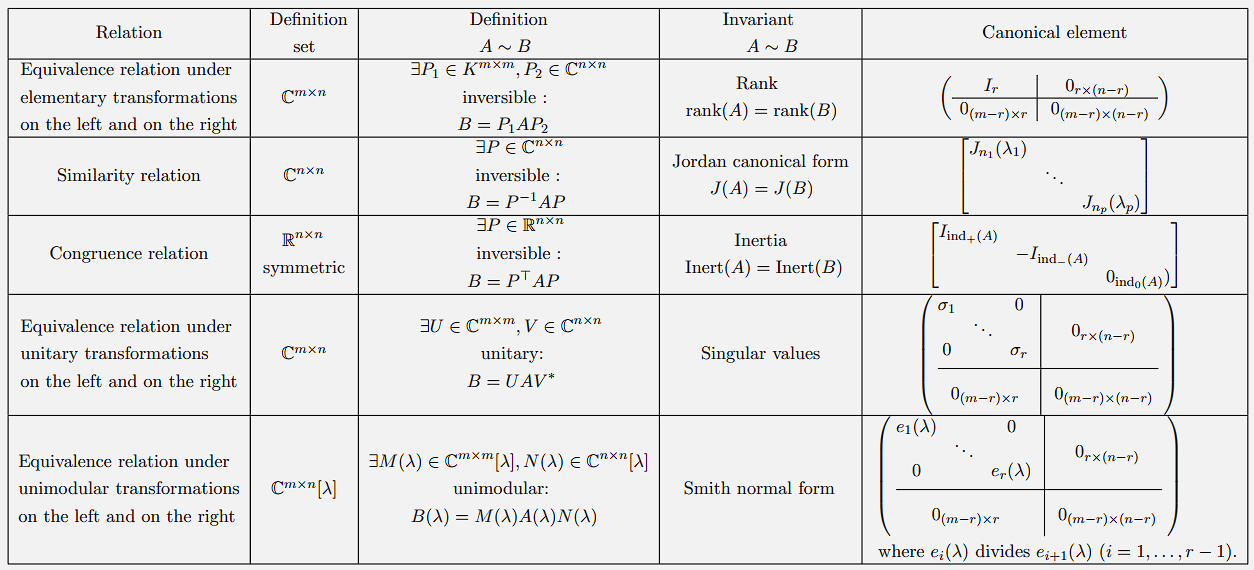
\includegraphics[width=\textwidth]{img/summary.png}
\end{figure}
\end{document}